\documentclass[11pt]{article}

\usepackage{a4wide}
\usepackage{mathptm}
\usepackage{xspace}
\usepackage{amsmath}
\usepackage{graphicx}
% 代码样式
\usepackage{algorithm}


% 参考文献引用上标,但是这个是英文reference
% \usepackage[super,square]{natbib}
\usepackage{algpseudocode}
\usepackage{tikz}
\usepackage{tkz-graph}
\usetikzlibrary{shapes.misc, positioning}
\usepackage{listings}
\usepackage{color}
% 设定页边距
\usepackage[top=2.5cm,bottom=2.5cm,left=2.5cm,right=2.5cm]{ geometry}
\usepackage[colorlinks = true,
            linkcolor = blue,
            urlcolor  = blue,
            citecolor = blue,
            anchorcolor = blue]{hyperref}
\usepackage{svg}
%设置首行缩进
\usepackage{indentfirst}
\setlength{\parindent}{2em }
\setlength{\parskip}{0pt }
%段前段后距离设置
%页眉和页脚%页眉和页脚
\definecolor{mauve}{rgb}{0.88, 0.69, 1.0}
% 创建一个新的命令,控制
\makeatletter
\def\@cite#1#2{\textsuperscript{[{#1\if@tempswa , #2\fi}]}}
\makeatother


\lstset{frame=tb,
  language=Java,
  aboveskip=3mm,
  belowskip=3mm,
  showstringspaces=false,
  columns=flexible,
  basicstyle={\small\ttfamily},
  numbers=left,
  numberstyle=\tiny\color{gray},
  keywordstyle=\color{blue},
  commentstyle=\color{dkgreen},
  stringstyle=\color{mauve},
  breaklines=true,
  breakatwhitespace=true,
  tabsize=3
}

% Xelatex中文宏包
\usepackage{CTEX}
\begin{document}

\title{MarkLogic调研}

\author{@rh01 https://github.com/rh01}

\date{}

\maketitle

\begin{abstract}

  多模型数据库(Multi-Model Database)是新一代的数据库,与只支持单一数据模型的传统数据库有所不同,多模型数据库是一种在统一、
  综合的平台下同时支持多种不同的数据模型的数据库,这些数据模型可包括传统的关系模型和NoSQL数据模型,并且多模型数据库
  具有自己一种或多种的查询语言,并不仅仅依赖于传统的SQL查询语言,这使得数据组织、管理和操作变得十分的简单和便捷。
  在企业中,拥有结构良好的数据和基于NoSQL技术的综合数据平台对用户是有益的 \cite{lu2017multi} ,
  这种方法显著地降低了集成,迁移,开发,维护和运营等问题.
  因此,在本论文中,我们将介绍多数据模型的数据库代表-MarkLogic, 将会介绍它的底层架构,所支持的数据模型,以及在底层和顶层如何访问、管理和操作
  数据,最后设计Benchmark来对MarkLogic进行评测,并与文档数据库MongoDB进行比较.

  \noindent 关键字:Multi-Model Database; MarkLogic; MongoDB

\end{abstract}



%\input{commands}

\section{MarkLogic简介}
\label{sec:introduction}

MarkLogic

\begin{itemize}
  
\item A brief motivation and introduction to the topic of the project.

\item Discuss history of the technology, mention related technologies (if relevant).

\item A brief account of the results that have been obtained in the project.

\item A one paragraph overview at the end, explaining how the rest of
  the report has been organised.

\end{itemize}

\noindent
This rest of this report is organised as follows:
Section~\ref{sec:background} gives an ....



\section{MarkLogic重要特性}
\label{sec:background}

About 4 pages that introduces in (sufficient) depth the key concepts
and architecture of the technology.  May use a running example to
introduce the technology.

This part and other parts of the report probably needs to refer to
figures. Figure~\ref{fig:framework} from \cite{brown:96} just
illustrates how figure can be included in the report.

\begin{figure}
  \centering
  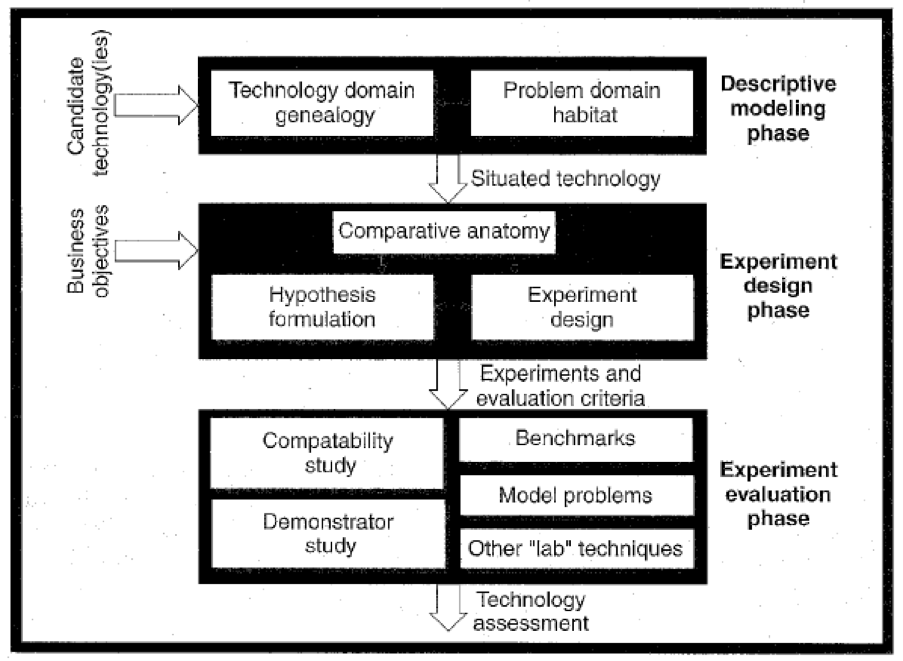
\includegraphics[scale=0.5]{figs/framework.png}
  \caption{Software technology evaluation framework.}
  \label{fig:framework}
\end{figure}


\section{编程API}
\label{sec:api}

About 5 pages that gives:

\begin{enumerate}
  
\item High-level view of the demonstrator and its purpose.

\item Details of how the demonstrator has been implemented.

\item May involve presentation of code snippets.

\end{enumerate}

The example below shows how you may include code. There are similar
styles for many other langages - in case you do not use Java in your
project. You can wrap the listing into a figure in case you need to
refer to it. How to create a figure was shown in Section~\ref{sec:background}.
  
\lstinputlisting[language=java]{code/BoksVolum.java}


\section{测试环境和测试结果}
\label{sec:experiments}

About 3 pages that:

\begin{description}

\item[Describes] the software used to establish the test-bed and for implementing the demonstrator prototype.

\item[Explains] what experiments have been done and the results.

\end{description}

For some reports you may have to include a table with experimental
results are other kinds of tables that for instance compares
technologies. Table~\ref{tab:results} gives an example of how to create a table.

\begin{table}
\centering
\begin{tabular}{llrrrrrr}
  Config & Property & States & Edges & Peak & E-Time & C-Time & T-Time
  \\ \hline \hline
22-2 & A   &    7,944  &   22,419  &  6.6  \%  &  7 ms & 42.9\% &  485.7\% \\   
22-2 & A   &    7,944  &   22,419  &  6.6  \%  &  7 ms & 42.9\% &  471.4\% \\   
30-2 & B   &   14,672  &   41,611  &  4.9  \%  & 14 ms & 42.9\% &  464.3\% \\   
30-2 & C   &   14,672  &   41,611  &  4.9  \%  & 15 ms & 40.0\% &  420.0\% \\ \hline
10-3 & D   &   24,052  &   98,671  & 19.8  \%  & 35 ms & 31.4\% &  285.7\% \\   
10-3 & E   &   24,052  &   98,671  & 19.8  \%  & 35 ms & 34.3\% &  308.6\% \\
\hline \hline
\end{tabular}
\caption{Selected experimental results on the communication protocol example.}
\label{tab:results}
\end{table}


\section{结论}

Concludes on the project, including the technology, its maturity,
learning curve, and quality of the documentation.

The references used throughput the report should constitute a well
chosen set of references, suitable for someone interesting in learning
about the technology.



\bibliographystyle{plain}
\bibliography{report}


\end{document}
